
% This LaTeX was auto-generated from MATLAB code.
% To make changes, update the MATLAB code and republish this document.

\documentclass{article}
\usepackage{graphicx}
\usepackage{color}

\sloppy
\definecolor{lightgray}{gray}{0.5}
\setlength{\parindent}{0pt}

\begin{document}

    
    

\section*{4. Interpolants, projections, and aliasing}

\begin{verbatim}
ATAPformats
\end{verbatim}
\begin{par}

Suppose $f(x)$ is a Lipschitz continuous function on $[-1,1]$ with
Chebyshev series coefficients $\{a_k\}$ as in Theorem 3.1,
$$ f(x) = \sum_{k=0}^\infty  a_k T_k(x). \eqno (4.1) $$
One approximation to $f$ in
${\cal P}_n$ is the polynomial obtained by {\bf interpolation} in
Chebyshev points:
$$ p_n(x) = \sum_{k=0}^n c_k T_k(x). \eqno (4.2) $$
Another is the polynomial obtained by {\em truncation} or {\em projection}
of the series to degree $n$,
whose coefficients through degree $n$ are the same as those of
$f$ itself:
$$ f_n(x) = \sum_{k=0}^n a_k T_k(x). \eqno (4.3) $$
The relationship of the Chebyshev coefficients of $f_n$ to those of $f$ is
obvious, and in a moment we shall see that the Chebyshev coefficients of
$p_n$ have simple expressions too. In computational work generally, and
in particular in Chebfun, the polynomials $\{p_n\}$ are usually almost as
good approximations to $f$ as the polynomials $\{f_n\}$, and easier to
work with, since one does not need to evaluate the integral (3.12).  The
polynomials $\{f_n\}$, on the other hand, are also interesting.  In this
book, most of our computations will make use of $\{p_n\}$, but many of
our theorems will treat both cases.  A typical example is Theorem 8.2,
which asserts that if $f$ is analytic on $[-1,1]$, then both $\|f-f_n\|$
and $\|f-p_n\|$ decrease geometrically to 0 as $n\to\infty$.

\end{par} \vspace{1em}
\begin{par}
The key to understanding $\{c_k\}$ is the phenomenon of \textit{aliasing,} a term that originated with radio engineers early in the 20th century. On the $(n+1)\kern -3pt$ -point Chebyshev grid, it is obvious that any function $f$ is indistinguishable from a polynomial of degree $n$. But something more is true: any Chebyshev polynomial $T_N$, no matter how big $N$ is, is indistinguishable on the grid from a \textit{single} Chebyshev polynomial $T_m$ for some $m$ with $0\le m \le n$.  We state this as a theorem.
\end{par} \vspace{1em}
\begin{par}
\textbf{Theorem 4.1. Aliasing of Chebyshev polynomials.} \textit{For any $n\ge 1$ and $0\le m \le n$, the following Chebyshev polynomials take the same values on the $(n+1)$-point Chebyshev grid:}
\end{par} \vspace{1em}
\begin{par}
$~~~~$ $T_m,\; T_{2n-m},\; T_{2n+m},\; T_{4n-m},\; T_{4n+m}, \; T_{6n-m},\dots.$
\end{par} \vspace{1em}
\begin{par}
\textit{Equivalently, for any $k\ge 0 $, $T_k$ takes the same value on the grid as} $T_m$ \textit{with} $$ m = | (k+n-1) (\hbox{mod\kern .7pt} 2n) - (n-1)| , \eqno (4.4) $$ \textit{a number in the range $0\le m \le n$.}
\end{par} \vspace{1em}
\begin{par}
\textit{Proof.} Recall from (2.1) and (3.8) that Chebyshev polynomials on $[-1,1]$ are related to monomials on the unit circle by $T_m(x) = (z^m + z^{-m})/2$, and Chebyshev points are related to $(2n)\kern -3pt$ th roots of unity by $x_m = (z_m^{} + z_m^{-1})/2$. It follows that the first assertion of the theorem is equivalent to the statement that the following functions take the same values at the $(2n)\kern -3pt$ th roots of unity:
\end{par} \vspace{1em}
\begin{par}
$~~~~$ $z^m+z^{-m},~ z^{2n-m} +z^{m-2n},~ z^{2n+m}+z^{-2n-m},\dots.$
\end{par} \vspace{1em}
\begin{par}
Inspection of the exponents shows that in every case, modulo $2n$, we have one exponent equal to $+m$ and the other to $-m$. The conclusion now follows from the elementary phenomenon of aliasing of monomials on the unit circle: at the $(2n)\kern -3pt$ th roots of unity, $z^{2\nu n} = 1$ for any integer $\nu$.
\end{par} \vspace{1em}
\begin{par}
For the second assertion (4.4), suppose first that $0\le k\,(\hbox{mod\kern .7pt} 2n) \le n$. Then $n-1 \le (k+n-1)(\hbox{mod\kern .7pt} 2n) \le 2n-1$, so (4.4) reduces to $m = k\,(\hbox{mod\kern .7pt} 2n)$, with $0\le m \le n$, and we have just shown that this implies that $T_k$ and $T_m$ take the same values on the grid.  On the other hand, suppose that $n+1\le k\,(\hbox{mod\kern .7pt} 2n) \le 2n-1$. Then $0\le (k+n-1)(\hbox{mod\kern .7pt} 2n) \le n-2 $, so the absolute value becomes a negation and (4.4) reduces to $m = -k\,(\hbox{mod\kern .7pt} 2n)$, with $1\le m \le n$. Again we have just shown that this implies that $T_k$ and $T_m$ take the same values on the grid. $~\hbox{\vrule width 2.5pt depth 2.5 pt height 3.5 pt}$
\end{par} \vspace{1em}
\begin{par}
Here is a numerical illustration of Theorem 4.1. Taking $n=4$, let \texttt{X} be the Chebyshev grid with $n+1$ points, and let $T\{1\},\dots,T\{10\}$ be the first ten Chebyshev polynomials:
\end{par} \vspace{1em}
\begin{par}
 \vskip -2em 
\end{par} \vspace{1em}
\begin{verbatim}
n = 4; X = chebpts(n+1);
for k = 1:10, T{k} = chebpoly(k); end
\end{verbatim}
\begin{par}
Then $T_3$ and $T_5$ are the same on the grid:
\end{par} \vspace{1em}
\begin{par}
 \vskip -2em 
\end{par} \vspace{1em}
\begin{verbatim}
disp([T{3}(X) T{5}(X)])
\end{verbatim}

        \color{lightgray} \begin{verbatim}  -1.000000000000000  -1.000000000000000
   0.707106781186548   0.707106781186547
                   0                   0
  -0.707106781186548  -0.707106781186547
   1.000000000000000   1.000000000000000
\end{verbatim} \color{black}
    \begin{par}
So are $T_1$, $T_7$, and $T_9$:
\end{par} \vspace{1em}
\begin{par}
 \vskip -2em 
\end{par} \vspace{1em}
\begin{verbatim}
disp([T{1}(X) T{7}(X) T{9}(X)])
\end{verbatim}

        \color{lightgray} \begin{verbatim}  -1.000000000000000  -1.000000000000000  -1.000000000000000
  -0.707106781186547  -0.707106781186548  -0.707106781186547
                   0                   0                   0
   0.707106781186547   0.707106781186548   0.707106781186547
   1.000000000000000   1.000000000000000   1.000000000000000
\end{verbatim} \color{black}
    \begin{par}
As a corollary of Theorem 4.1, we can now derive the connection between $\{a_k\}$ and $\{c_k\}$. The following result can be found in [Clenshaw \& Curtis 1960].
\end{par} \vspace{1em}
\begin{par}
 \em
{\bf Theorem 4.2. Aliasing formula for Chebyshev coefficients.}
Let $f$ be Lipschitz continuous on $[-1,1]$, and let
$p_n$ be its Chebyshev interpolant in ${\cal P}_n$,
$n \ge 1$.  Let $\{a_k\}$ and $\{c_k\}$ be the
Chebyshev coefficients of $f$ and $p_n$, respectively.  Then
$$ c_0 = a_0 + a_{2n} + a_{4n} + \cdots, \eqno (4.5) $$
$$ c_n = a_n + a_{3n} + a_{5n} + \cdots, \eqno (4.6) $$
and for $1 \le k \le n-1$,
$$ c_k = a_k + (a_{k+2n} + a_{k+4n}+\cdots) +
(a_{-k+2n}+ a_{-k+4n}+\cdots).\eqno (4.7)  $$
\vspace{-1.5em} 
\end{par} \vspace{1em}
\begin{par}
\textit{Proof.}  By Theorem 3.1, $f$ has a unique Chebyshev series (3.11), and it converges absolutely.  Thus we can rearrange the terms of the series without affecting convergence, and in particular, each of the three series expansions written above converges since they correspond to the Chebyshev series (3.11) evaluated at $x=1$, So the formulas (4.5)--(4.7) do indeed define certain numbers $c_0,\dots, c_n$. Taking these numbers as coefficients multiplied by the corresponding Chebyshev polynomials $T_0, \dots, T_n$ gives us a polynomial of degree $n$.  By Theorem 4.1, this polynomial takes the same values as $f$ at each point of the Chebyshev grid. Thus it is the unique interpolant $p_n\in {\cal P}_n$. $~\hbox{\vrule width 2.5pt depth 2.5 pt height 3.5 pt}$
\end{par} \vspace{1em}
\begin{par}
We can summarize Theorem 4.2 as follows.  On the $(n+1)$-point grid, any function $f$ is indistinguishable from a polynomial of degree $n$. In particular, the Chebyshev series of the polynomial interpolant to $f$ is obtained by reassigning all the Chebyshev coefficients in the infinite series for $f$ to their aliases of degrees 0 through $n$.
\end{par} \vspace{1em}
\begin{par}
As a corollary, Theorems 4.1 and 4.2 give us absolutely convergent series for $f-f_n$ and $f-p_n$, which we shall exploit in Chapters 7 and 8: $$ f(x) - f_n(x) = \sum_{k=n+1}^\infty a_k T_k(x), \eqno (4.8) $$ $$ f(x) - p_n(x) = \sum_{k=n+1}^\infty a_k ( T_k(x) - T_m(x)), \eqno (4.9) $$ where $m = m(k,n)$ is given by (4.4).
\end{par} \vspace{1em}
\begin{par}
To illustrate Theorem 4.2, here is the function $f(x) = \tanh(4x-1)$ (solid) and its degree 4 Chebyshev interpolant $p_4(x)$ (dashed):
\end{par} \vspace{1em}
\begin{par}
 \vskip -2em 
\end{par} \vspace{1em}
\begin{verbatim}
x = chebfun('x');
f = tanh(4*x-1);
n = 4; pn = chebfun(f,n+1);
hold off, plot(f), hold on, plot(pn,'.--r')
FS = 'fontsize';
title('A function f and its degree 4 interpolant p_4',FS,9)
\end{verbatim}

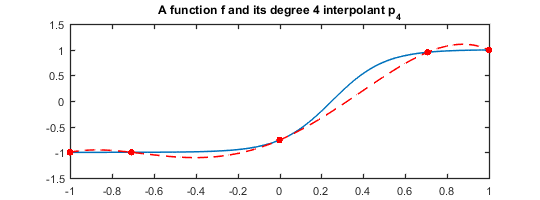
\includegraphics [width=4in]{chap4_01.png}
\begin{par}
 \vskip 1pt 
\end{par} \vspace{1em}
\begin{par}
The first 5 Chebyshev coefficients of $f$,
\end{par} \vspace{1em}
\begin{par}
 \vskip -2em 
\end{par} \vspace{1em}
\begin{verbatim}
a = chebpoly(f); a = a(end:-1:1)'; a(1:n+1)
\end{verbatim}

        \color{lightgray} \begin{verbatim}ans =
  -0.166584582703135
   1.193005991160944
   0.278438064117869
  -0.239362401056012
  -0.176961398392888
\end{verbatim} \color{black}
    \begin{par}
are different from the Chebyshev coefficients of $p_n$,
\end{par} \vspace{1em}
\begin{par}
 \vskip -2em 
\end{par} \vspace{1em}
\begin{verbatim}
c = chebpoly(pn); c = c(end:-1:1)'
\end{verbatim}

        \color{lightgray} \begin{verbatim}c =
  -0.203351068209675
   1.187719968517890
   0.379583465333916
  -0.190237989543227
  -0.178659622412174
\end{verbatim} \color{black}
    \begin{par}
As asserted in (4.5) and (4.6), the coefficients $c_0$ and $c_n$ are given by sums of coefficients $a_k$ with a stride of $2n$:
\end{par} \vspace{1em}
\begin{par}
 \vskip -2em 
\end{par} \vspace{1em}
\begin{verbatim}
c0 = sum(a(1:2*n:end)), cn = sum(a(n+1:2*n:end))
\end{verbatim}

        \color{lightgray} \begin{verbatim}c0 =
  -0.203351068209675
cn =
  -0.178659622412174
\end{verbatim} \color{black}
    \begin{par}
As asserted in (4.7), the coefficients $c_1$ through $c_{n-1}$ involve two sums of this kind:
\end{par} \vspace{1em}
\begin{par}
 \vskip -2em 
\end{par} \vspace{1em}
\begin{verbatim}
for k = 1:n-1
  ck = sum(a(1+k:2*n:end)) + sum(a(1-k+2*n:2*n:end))
end
\end{verbatim}

        \color{lightgray} \begin{verbatim}ck =
   1.187719968517890
ck =
   0.379583465333916
ck =
  -0.190237989543227
\end{verbatim} \color{black}
    \begin{par}
Following up on the last figure, how does the truncated series $f_n$ compare with the interpolant $p_n$ as an approximation to $f$?  Chebfun includes a \texttt{'trunc'} option for computing $f_n$, which we now add to the plot as a dot-dash line:
\end{par} \vspace{1em}
\begin{par}
 \vskip -2em 
\end{par} \vspace{1em}
\begin{verbatim}
fn = chebfun(f,'trunc',n+1);
plot(fn,'-.g')
title('Function f, interpolant p_4, projected approximant f_4',FS,9)
\end{verbatim}

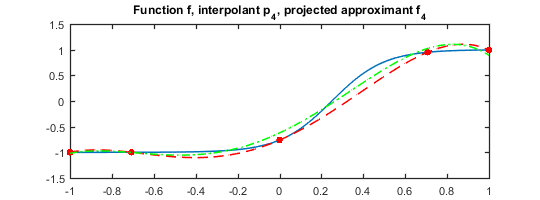
\includegraphics [width=4in]{chap4_02.png}
\begin{par}
 \vskip 1pt 
\end{par} \vspace{1em}
\begin{par}
Here are the errors $f-f_n$ and $f-p_n$:
\end{par} \vspace{1em}
\begin{par}
 \vskip -2em 
\end{par} \vspace{1em}
\begin{verbatim}
hold off
subplot(1,2,1), plot(f-fn,'g'), ylim(.38*[-1 1])
title('Error in projection f-f_4',FS,9)
subplot(1,2,2), plot(f-pn,'r'), ylim(.38*[-1 1])
title('Error in interpolant f-p_4',FS,9)
\end{verbatim}

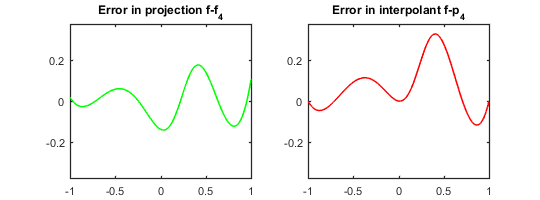
\includegraphics [width=4in]{chap4_03.png}
\begin{par}
 \vskip 1pt 
\end{par} \vspace{1em}
\begin{par}
Here is the analogous plot with $n=4$ increased to $24$:
\end{par} \vspace{1em}
\begin{par}
 \vskip -2em 
\end{par} \vspace{1em}
\begin{verbatim}
n = 24; pn = chebfun(f,n+1);
fn = chebfun(f,'trunc',n+1);
subplot(1,2,1), plot(f-fn,'g'), ylim(.0005*[-1 1])
title('Error in projection f-f_{24}',FS,9)
subplot(1,2,2), plot(f-pn,'r'), ylim(.0005*[-1 1])
title('Error in interpolant f-p_{24}',FS,9)
\end{verbatim}

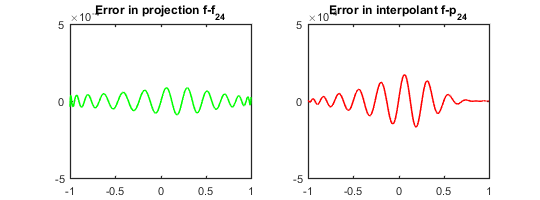
\includegraphics [width=4in]{chap4_04.png}
\begin{par}
 \vskip 1pt 
\end{par} \vspace{1em}
\begin{par}
On the basis of plots like these, one might speculate that $f_n$ may often be a better approximation than $p_n$, but that the difference is small.  This is indeed the case, as we shall confirm in Theorems 7.2 and 8.2, both of which suggest a difference of a factor of 2, and Theorem 16.1, which suggests a factor of $\pi/2$.
\end{par} \vspace{1em}
\begin{par}

Let us review where we stand. We have considered Chebyshev
interpolants (Chapter 2) and Chebyshev expansions (Chapter 3) for a
Lipschitz continuous function $f(x)$ defined on $[-1,1]$. Mathematically
speaking, each coefficient of a Chebyshev expansion is equal to the value
of the integral (3.12).  This formula, however, is not needed for
effective polynomial approximation, since Chebyshev interpolants are
nearly as accurate as projections. Chebfun readily computes
Chebyshev coefficients of polynomial interpolants, and this is done not
by evaluating the integral but by taking the FFT of the sample values in
Chebyshev points. If the degree of the interpolant is high enough that
the polynomial matches $f$ to machine precision, then the Chebyshev
coefficients will match too.

\end{par} \vspace{1em}
\begin{par}

\begin{displaymath}
\framebox[4.7in][c]{\parbox{4.5in}{\vspace{2pt}\sl
{\sc Summary of Chapter 4.}
Two excellent methods of approximating a function $f$ on $[-1,1]$ by a
polynomial are truncation of its Chebyshev series, also known as
projection, and interpolation in
Chebyshev points.  The Chebyshev interpolant is the polynomial obtained
by reassigning contributions of degree $>n$ in the Chebyshev series to
their aliases of degree ${\le}\kern 1pt n$. The two approximations are
typically within a factor of\/ $2$ of each other in
accuracy.\vspace{2pt}}}
\end{displaymath}

\end{par} \vspace{1em}
\begin{par}
\smallskip\small\parskip=2pt
{\bf Exercise 4.1.  Node polynomial for Chebyshev points.} Show using
Theorem 4.1 that $p(x) = 2^{-n}(T_{n+1}(x) - T_{n-1}(x))$ is the unique
monic polynomial in ${\cal P}_{n+1}$ with zeros at the $n+1$ Chebyshev
points (2.2).
\par
{\bf Exercise 4.2.  Examples of aliasing.} (a) On the $(n+1)$-point
Chebyshev grid with $n = 20$, which Chebyshev polynomials $T_k$ take the
same values as $T_5$?  (b) Use Chebfun to draw plots illustrating some of
these intersections.
\par
{\bf Exercise 4.3.  Aliasing in roots of unity.}  For each $n\ge 0$, let
$p_n\in {\cal P}_n$ be the degree $n$ polynomial interpolant to the
function $f(z) = z^{-1}$ at the $(n+1)$st roots of unity on the unit
circle in the $z$-plane.   Use the aliasing observation of the proof of
Theorem 4.1 to prove that in the closed unit disk of complex numbers
$z$ with $|z|\le 1$, there is one and only one value $z$ for which $p_n$
converges to $f$ as $n\to\infty$.  (This example comes
from $\hbox{[M\'eray}$ 1884].)
\par
{\bf Exercise 4.4.  Fooling the Chebfun constructor.}  (a) Construct the
Matlab anonymous function \verb|f = @(M) chebfun(@(x) 1+exp(-(M*(x-0.4)).^4))|
and plot {\tt f(10)} and {\tt f(100)}.  This function has a narrow spike
of width proportional to $1/M$.  Confirm this by comparing {\tt
sum(f(10))} and {\tt sum(f(100))}. (b) Plot {\tt length(f(M))} as a
function of $M$ for $M = 1,2,3,\dots,$ going into the region where the
length becomes~$1$. What do you think is happening? (c) Let {\tt Mmax} be
the largest integer for which the constructor behaves normally and
execute {\tt semilogy(f(Mmax)-1,'interval',[.3 .5])}. Superimpose on this
plot information to show the locations of the points returned by {\tt
chebpts(9)}, which is the default initial grid on which Chebfun samples a
function.  Explain how this result fits with (b). (d) Now for {\tt np}
taking values 17, 33, 65, 129, execute {\tt chebfunpref('minsamples',np)}
and {\tt length(f(np))}, and plot the Chebyshev points on your semilog
plot of (c).  The {\tt minsamples} flag forces Chebfun to sample the
function at the indicated number of points.  How do these results match
your observations of (b) and (c)?  When you're done, be sure to return
Chebfun to its default state with {\tt chebfunpref('factory')}.
\par
{\bf Exercise 4.5.  Relative precision.}  Try Exercise 4.4 again but
without the ``1+'' in the definition of {\tt f}.  The value of {\tt Mmax}
will be different, and the reason has to do with Chebfun's aim of
constructing each function to about 15 digits of relative precision, not
absolute.  Can you figure out what is happening and explain it
quantitatively?
\par
{\bf Exercise 4.6.  Chebfun computation of truncations.} In the text we
computed Chebyshev truncations of $f(x) = \tanh(4x-1)$ using the {\tt
'trunc'} flag in the Chebfun constructor. Another method is to compute
all the Chebyshev coefficients of $f$ and then truncate the series.
Compute $f_4$ by this method and verify that the results agree to machine
precision.
\par
{\bf Exercise 4.7.  When projection equals interpolation.}
Sometimes the projection $f_n$ and the interpolant $p_n$ are
identical, even though both differ from $f$.  Characterize exactly
when this occurs, and give an example with $n=3$.
\par

\end{par} \vspace{1em}



\end{document}
    
